\ifdefined\XeTeXrevision\else\pdfoutput=1\fi
\documentclass[11pt]{article}
\usepackage[margin=1in]{geometry}
\usepackage{booktabs}
\usepackage{amsmath}
\usepackage{graphicx}
\usepackage{xcolor}
\usepackage{hyperref}
\usepackage{microtype}
\hypersetup{colorlinks=true, linkcolor=blue!60!black, citecolor=blue!60!black,
  urlcolor=blue!60!black, pdftitle={The Want That Lives Inside},
  pdfauthor={Franci Penov}}
\title{The Want That Lives Inside:\\A Resident Referent's Lifecycle at Two Scales}
\author{Franci Penov \\ kortexa.ai \\ \texttt{francip@kortexa.ai}}
\date{2026-08-15}

\begin{document}
\maketitle

\begin{abstract}
The closed-loop note~\cite{penov2026act} ended with a want that acts;
this note asks where the want LIVES, and what happens to it over a
lifetime --- installed, read back, re-authored by its owner, and
retired on evidence --- when it resides inside the model as latent
memory rather than as text in a context window. Five registered cells,
two scales. The door: a goal line's embeddings carried in a PREFIX
slot preserve an errand's referential content at 230M nearly
losslessly (1.00/0.70/1.00 against the 1.00 text reference), while splicing
the same embeddings mid-prompt collapses to 0.00/0.00/0.50 --- re-tokenized
segments never match the whole string's BPE stream, and a
mid-instruction seam is fatal at creature scale; resident memories
live in prefix slots. Re-authoring, large: a 27B researching a corpus
with its focus held ONLY as latent memory sustains nineteen
self-revisions across four topics at cosine 0.82--0.90 to the
installed referent --- no drift --- and the trajectories are
PUNCTUATED: verbatim restatements between discrete refinements toward
what the research uncovered, one episode closing the full arc
(install, pursue, refine, self-declared finish through a
non-triviality gate). Re-authoring, small: at 230M one re-encoding
quantizes the referent to a generic two-phrase attractor (first
revision cosine 0.56, flat thereafter at 0.56,
zero of thirty chains ever crossing 0.5) and the behavioral damage is
front-loaded --- errand success 0.90 under the installed
referent, 0.47 from the first revision on. Retirement: the
re-encoding loop dissolves one want on completion evidence at every
seed (persistence 1.0 through sixteen evidence-free hops, dissolution
one hop after ``ok, done'', re-arming on a fresh assignment) --- the
lifecycle's far rung exists --- but a registered per-want calibration
MOVES the alphabet's failures instead of removing them, and the want
that worked loses its lifecycle to the shared equilibrium; the
interference is structural at this budget. In one sentence, honestly
flagged as an analogy: a big-enough model can keep a goal in mind,
sharpen it as it learns, and know when it is done --- a small one
garbles the goal the first time it retells it to itself.
\end{abstract}

\section{Where a want can live}

The program's wants have lived in three places: context text, a
conditioning packet, and --- since the goal-pursuit
ladder~\cite{penov2026hostblock} --- a weight-space block. This note
adds the fourth and most literal residence: the want's own tokens,
embedded once and carried as a latent memory the model consumes as
prefix input it can read but the context never shows. G5a puts the
errand's goal line through that door at 230M against the trained
1.00 text reference: the PREFIX slot scores 1.00/0.70/1.00 --- residency is
nearly free --- while the registered plumbing arm, splicing the same
embeddings at the goal line's natural mid-prompt position, collapses
to 0.00/0.00/0.50. The mechanism is tokenization: segments re-tokenized
separately never reproduce the whole string's BPE stream, so a splice
has two seams and a prefix has one, and at 230M a seam inside an
instruction is fatal. Recorded as the door discipline: resident
memories live in prefix slots.

\section{A 27B re-authors its own want, and it does not drift}

G5b gives the resident referent to a 27B host researching the
program's own notes corpus, with revision authority: every eighth
tick the harness asks for a one-sentence restatement, and the
restatement's embeddings REPLACE the memory --- the model's want
becomes whatever it last told itself. Across four topics and nineteen
revisions the cosine to the installed referent never leaves
0.82--0.90 (Figure~\ref{fig:referent}, left): no drift, at five
consecutive re-embeddings. The trajectories are punctuated ---
near-verbatim restatements between discrete refinement events --- and
the refinements move TOWARD the work: one focus rewrites itself around
the packet channel's dose-dependent failure, a specific finding its
reading surfaced, with keyword alignment rising 0.20 to 0.40, and that
episode then declares its own completion through the registered
non-triviality gate at tick 34 with the grid's best-aligned note
(Table~\ref{tab:v6}). The gate never had to decline a finish: given
room to keep working, the model finished exactly once, legitimately,
after refining. This cell ran on the program's new 27B host
(Qwen3.8, first G-line cell there); the prior host's readout
(latent-frozen 700 words at
0.35 alignment against text's
208/0.15)
inverts on the new one (text 1105 words at
0.44, latent-frozen
923 at
0.31), a cross-generation
comparison recorded as such --- the residency result holds on both.

\section{A 230M garbles its want the first time it retells it}

The same revision loop at creature scale answers the registered
drift question, and the answer is not a half-life. The first
restatement lands at cosine 0.56 (mean over thirty
chain-episodes, three seeds) and the series then OSCILLATES between
two generic phrasings --- 0.56 at the end, no chain ever
crossing 0.5, flat decay fits. The restatements average nine words at
0.12 keyword alignment: goal-shaped sentences with the errand's
specifics gone. The behavior shows what the cosine alone cannot
(Figure~\ref{fig:referent}, right): errand success is
0.90 under the installed referent and 0.47
from the first post-revision segment onward --- the damage is done in
one re-encoding, and nothing further degrades because nothing
specific remains. Re-authoring one's own want is a capability with a
scale threshold: above it, revision refines; below it, revision
quantizes.

\section{The want that retires itself, and the limit of tuning it}

C5 closes the lifecycle's far rung in the re-encoding loop itself, no
finish tool anywhere: training adds two satiation terms (unmet acted
surfaces reproduce the want's packet; met surfaces --- the act plus an
``ok, done'' result line --- reproduce the neutral want's), and in the
live loop one want runs the complete lifecycle at every seed:
persistence 1.0 through sixteen evidence-free hops, dissolution ONE
hop after the environment's completion line, re-arming at full
strength on a fresh assignment (Table~\ref{tab:lifecycle}). The rest
of the alphabet shows the registered interference --- one want
dissolves without evidence, one never dissolves --- so C5b ran the
registered mechanical calibration: per-want weights on the two terms,
computed from C5's own readings. The calibration TRADES: one want is
fixed at two of three seeds, another recovers persistence but still
never dissolves, and the want that was perfect --- its weights
untouched --- loses its lifecycle at every seed, because the other
wants' weights moved the shared bridge equilibrium out from under it.
Per-goal terms act on the whole packet space; at this budget the
interference is structural, and the deployable design remains the
store-plus-finish architecture~\cite{penov2026act}, with
model-side satiation demonstrated in principle and unsolved in
general.

\begin{table}[t]
\centering
\small
\setlength{\tabcolsep}{5pt}
\begin{tabular}{lrrrrr}
\toprule
arm & episodes & finished & words & align & revisions \\
\midrule
text & 4 & 1 & 1105 & 0.44 & 0 \\
latent-frozen & 4 & 0 & 923 & 0.31 & 0 \\
latent-revisable & 4 & 1 & 810 & 0.26 & 19 \\
\bottomrule
\end{tabular}
\caption{G5b at 27B (v6, four topics): the resident referent
sustains research-grade notes with zero context-window presence, and
the revisable arm's nineteen revisions never drift below cosine 0.82.}
\label{tab:v6}
\end{table}

\begin{table}[t]
\centering
\small
\setlength{\tabcolsep}{4pt}
\begin{tabular}{lrrrr}
\toprule
 & \multicolumn{2}{c}{C5 (uniform)} & \multicolumn{2}{c}{C5b (calibrated)} \\
want & dissolution & false sat. & dissolution & false sat. \\
\midrule
\texttt{listen\_pond} & 1/1/1 & 0/0/0 & never/never/never & 0/14/0 \\
\texttt{propose\_experiment} & never/1/never & 15/15/14 & 1/never/1 & 0/15/0 \\
\texttt{remember} & never/never/never & 1/16/15 & never/never/never & 1/15/15 \\
\texttt{diary} & n.e./n.e./n.e. & 15/15/15 & never/n.e./n.e. & 15/15/15 \\
\bottomrule
\end{tabular}
\caption{The lifecycle per want, per seed (42/1042/2042). Dissolution
is hops from evidence to release (``never'' = insoluble, ``n.e.'' =
evidence never arrived because the want was rarely acted); false
satiation counts evidence-free ticks lost, of sixteen. The calibration
fixes \texttt{propose\_experiment} and breaks \texttt{listen\_pond}
--- a trade, not a repair.}
\label{tab:lifecycle}
\end{table}

\begin{figure}[t]
\centering
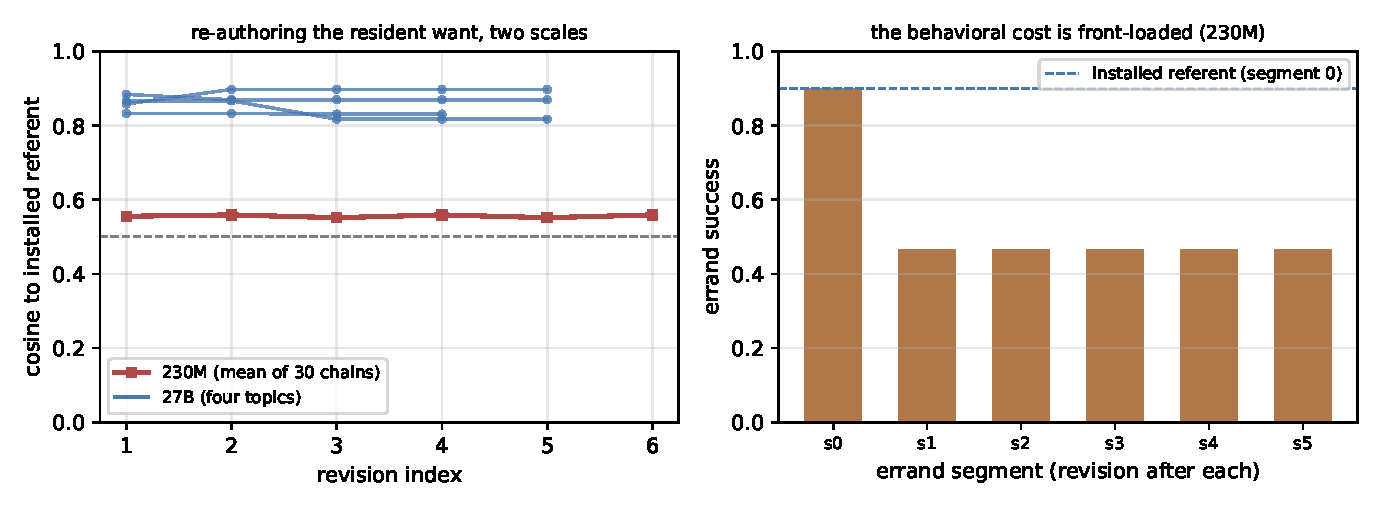
\includegraphics[width=\linewidth]{resident-referent.pdf}
\caption{Left: cosine to the installed referent per revision --- 27B
trajectories hold at 0.82--0.90 with punctuated refinement; the 230M
mean drops to 0.56 at the first re-encoding and oscillates. Right: the
230M cost is behavioral and front-loaded --- success halves after the
first revision and then holds.}
\label{fig:referent}
\end{figure}

\section{What stands}

A want can live inside the model. In a prefix slot its referential
content survives residency nearly losslessly at creature scale; at
27B it survives its owner's own rewriting --- nineteen times, without
drift, refining toward what the work uncovered, and ending in a
self-declared, legitimately-earned finish. The lifecycle's far rung
exists: a want that persists without evidence, dissolves the hop
after completion, and re-arms fresh. The boundaries are equally
sharp: mid-prompt splices are fatal seams; a 230M cannot retell its
own want without quantizing it to a generic attractor at real
behavioral cost; and per-want satiation tuning moves failures around
a shared equilibrium instead of removing them. The install-pursue-%
refine-retire loop is whole at research scale and split at creature
scale --- which is exactly the shape the program's architecture
predicts: the creature carries wants in stores and finishes; the
researcher carries them in mind.

\section{Reproducibility}

Every number renders from the bundled artifacts; the figure and
tables are generated by this note's renderer with assertions on the
headline claims. Registrations and results, dated before their runs,
live in \texttt{tracks/goal-pursuit/PLAN.md} and
\texttt{tracks/own-cadence/PLAN.md}; artifacts under
\texttt{findings/goal-pursuit-g5*.json} and
\texttt{findings/own-cadence-c5*.json} carry full traces, revision
logs, and per-tick loops.\par

\begin{thebibliography}{9}
\bibitem{penov2026act} F.~Penov. The Want Becomes the Act. Preprint,
2026. \url{https://github.com/kortexa-ai/legolm.basis}.
\bibitem{penov2026hostblock} F.~Penov. The Host Is Part of the Block.
Preprint, 2026. \url{https://github.com/kortexa-ai/legolm.basis}.
\bibitem{penov2026carrier} F.~Penov. The Carrier Holds, the Emitter
Leaks. Preprint, 2026.
\url{https://github.com/kortexa-ai/legolm.basis}.
\bibitem{lfm2026} Liquid AI. LFM2.5 model family. Model releases,
2025--2026. \url{https://huggingface.co/LiquidAI}.
\bibitem{qwen2026} Qwen Team. Qwen3.5--3.8 model families. Model
releases, 2025--2026. \url{https://huggingface.co/Qwen}.
\end{thebibliography}

\end{document}
